\section{Data Rate}
\todo[color=yellow]{When do I write the evaluation of the data rate? emidiately after the graph?}

Using ns-3 I built a simulation to evaluate effect of physical layer configuration on the achievable goodput between two nodes using IEEE 802.11ax Wi-Fi Netdevices in Adhoc Mode.
The setup consists of two nodes placed in static positions with a distance of \SI{20}{\metre}. I chose the short communication range to allow the use higher HE-\ac{MCS} values, which don't support long range transmissions due to path loss and shadowing effects.
Every node is eqipped with a Wi-Fi NetDevice with the following parameters: \ac{GI} of \SI{3200}{\nano\second}, a bandwidth of \SI{20}{\mega\hertz} and 2 spatial streams.
A Constant Rate Wifi Manager is used to set a constant data rate according to the fixed HE-\ac{MCS} for data, non-uniform and control data transmissions. The used frequency band is \SI{2.4}{\giga\hertz} or \SI{5}{\giga\hertz} as
higher frequencies are less resistant to shadowing and fading and a higher data rate is not needed for the \ac{WIC} use cases.
The Wi-Fi Netdevices operate in the frequency channels specified in \autoref{tab:frequencyChannels}, which can be used for
outdoor Wi-Fi communication in Germany \cite{GermanLaw}.

\begin{table}
	\centering
	\begin{tabular}{>{\centering}p{2cm}p{4cm}p{4cm}}
		\toprule
		\ac{BW} & Channel number \SI{2.4}{\giga\hertz} & Channel number \SI{2.4}{\giga\hertz}\\
		\midrule
		\SI{20}{\mega\hertz} & \num{1}&
		\num{100} \\
		\SI{40}{\mega\hertz} &
		\num{3}
		& \num{102} \\
		\SI{80}{\mega\hertz} &
		- & \num{106} \\
		\SI{160}{\mega\hertz} & -
		& \num{114} \\
		\bottomrule
	\end{tabular}
	\caption{Frequency Channels numbers for \SI{2.4}{\giga\hertz} and \SI{5}{\giga\hertz} for the different \ac{BW}s of the IEEE 802.11 standard \cite{noauthor_ieee_2021-1}, which can be used for
	outdoor communication \cite{GermanLaw}}
	\label{tab:frequencyChannels}
\end{table}



\todo[color=yellow]{UDP explanation?}
As the Wi-Fi standard implements ACKs for every packet, every lost packet is repeated until it is received or the number of retrys is
exceeded. Platooning Services are time critical and therefore the number of retrys should be as low as possible. This is why additional
retransmission mechanisms like TCP are not needed. Therefore, the chosen transport layer protocol is UDP.

One nodes operate a UDP server and the other one a UDP client. The client sends \SI{1000}{\byte} UDP packets to the server every \SI{0.0000001}{\second}. This packet interval
sorgt dafür, dass nach Start der Simulation the packet queue of the client is never empty. The server receives the packets and sends an ACK back to the client.

The simulation runs five times for \SI{5}{\second} for every physical layer configuration.
The goodput for every simulation run is calculated by dividing the number of received bytes at the UDP Server by the simulation time.
The goodput is then averaged over all simulation runs and the confidence interval with a confidence level of
\SI{95}{\percent} is calculated.

\todo{Überprüfung, PhyMonitor, Theoretical DataRates}
\subsubsection*{\acl{GI}}

In the first simulation I varied the \ac{GI} of the Wi-Fi Netdevices for different HE-\ac{MCS} values.
The results are shown in \autoref{fig:Data_rate_GI}. The achieved goodput is plotted against the theoretical data rate for the different \ac{GI} values.
The theoretical data rate is always higher than the achieved goodput of the UDP applications, because the channel is used for ACK and Adhoc Beacon transmissions as well. Due to
these additional transmissions the goodput is lower than the theoretical data rate. 

\begin{figure}%
	\centering
	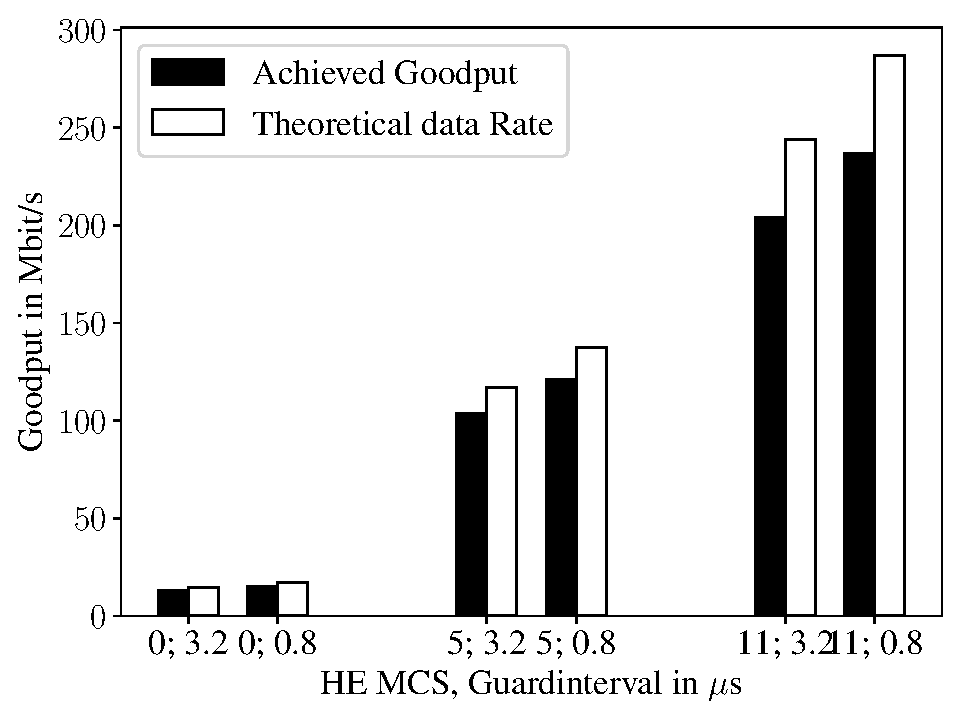
\includegraphics[width=0.95\textwidth]{figures/gi_dataRate_simulation.pdf}
	\caption{Achieved Goodput and theoretical Datarate of two WiFi 6 stations in Ad-Hoc Mode with \num{2} \ac{MIMO} streams and a bandwidth of \SI{80}{\mega\hertz} in regards to the number of \ac{MIMO} streams and the chosen \ac{MCS} and \ac{CR}}%
	\label{fig:Data_rate_GI}%
\end{figure}

atteninuation of bandwidth : 800ns : \SI{94}{\percent} \SI{89}{\percent} \SI{80}{\percent}

Factors apply for MCS0 but may also apply later

\begin{figure}%
	\centering
	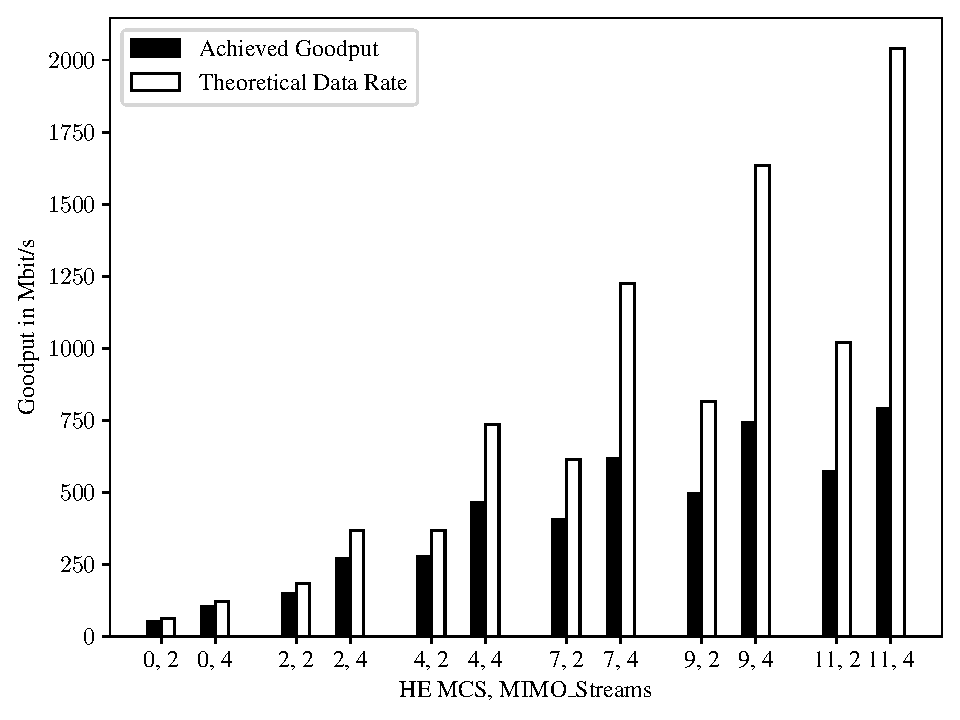
\includegraphics[width=0.95\textwidth]{figures/mimo_dataRate_simulation.pdf}
	\caption{Achieved Goodput and theoretical Datarate of two WiFi 6 stations in Ad-Hoc Mode with a \ac{GI} of \SI{3200}{\nano\second} and a bandwidth of \SI{80}{\mega\hertz} in regards to the number of \ac{MIMO} streams and the chosen \ac{MCS} and \ac{CR}}%
	\label{fig:Data_rate_Mimo}%
\end{figure}


\begin{figure}%
	\centering
	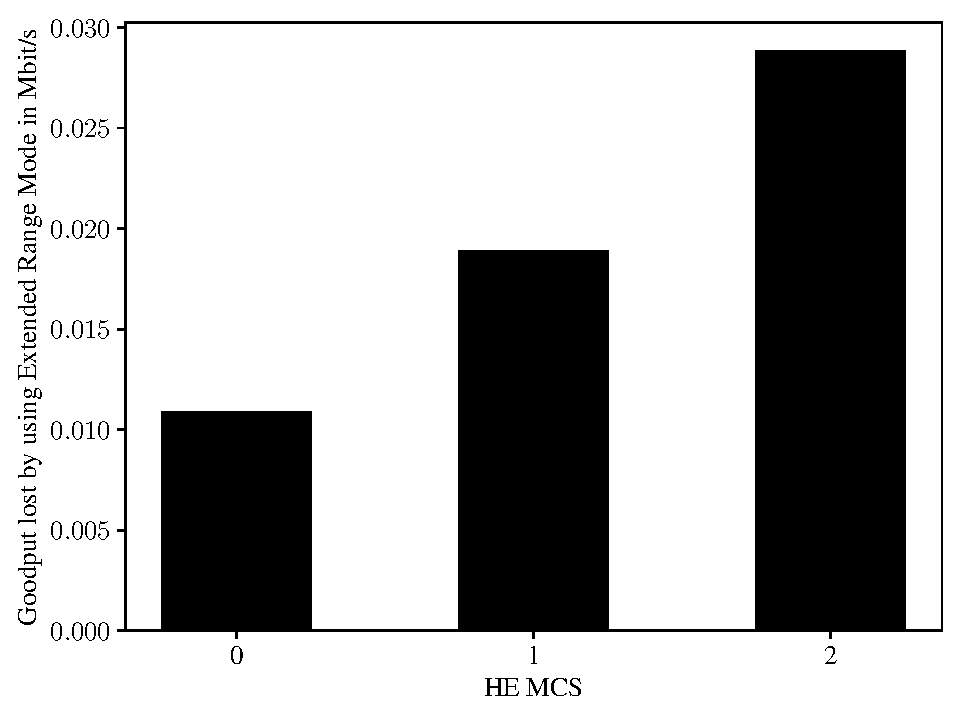
\includegraphics[width=0.95\textwidth]{figures/ER_dataRate_simulation.pdf}
	\caption{Achieved Goodput and theoretical Datarate of two WiFi 6 stations in Ad-Hoc Mode with a \ac{GI} of \SI{3200}{\nano\second} and a bandwidth of \SI{20}{\mega\hertz} in regards to the number of \ac{MIMO} streams and the chosen \ac{MCS} and \ac{CR}}%
	\label{fig:Data_rate_ER}%
\end{figure}

\todo{DataRate for STBC}
STBC and DCM * 2 payload / half data rate

\begin{figure}%
	\centering
	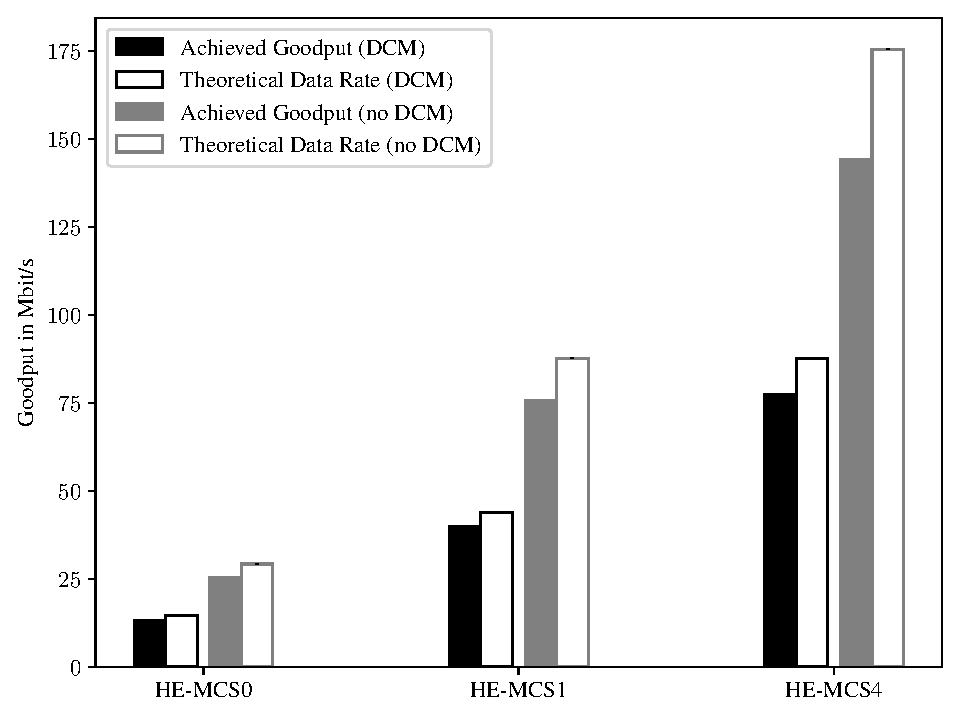
\includegraphics[width=0.95\textwidth]{figures/DCM_dataRate_simulation.pdf}
	\caption{Achieved Goodput and theoretical Datarate of two WiFi 6 stations in Ad-Hoc Mode with for IEEE 802.11ax physical layer parameters of a \ac{GI} of \SI{3200}{\nano\second}, a \ac{BW} of \SI{40}{\mega\hertz} and 2 spatial streams  in regards to the number of the chosen HE-\ac{MCS} value and whether \ac{DCM} is enabled}%
	\label{fig:Data_rate_DCM}%
\end{figure}


But Latency?
Latency is always based on Data Rate and Robustness

Data Rate and Robustness als related to oneanother

